\documentclass[a4paper,14pt]{article}

\usepackage{comment} % Para comentar várias linhas ao mesmo tempo

%matemática
\usepackage{amsmath}
\usepackage{amssymb}

%diagramação
\usepackage{extsizes}
\everymath{\displaystyle}
\usepackage{geometry}
\usepackage{fancyhdr}
\usepackage{multicol}
\usepackage{graphicx}
\usepackage[brazil]{babel}
\usepackage[shortlabels]{enumitem}
\usepackage{cancel}
\usepackage{textcomp}
\usepackage{tcolorbox}

%tabelas
\usepackage{array} % Para melhor formatação de tabelas
\usepackage{longtable}
\usepackage{booktabs}  % Para linhas horizontais mais bonitas
\usepackage{float}   % Para usar o modificador [H]
\usepackage{caption} % Para usar legendas em tabelas
\usepackage{wrapfig} % Para usar tabelas e figuras flutuantes


%tikzpicture
\begin{comment}
	\usepackage{tikz}
	\usepackage{scalerel}
	\usepackage{pict2e}
	\usepackage{tkz-euclide}
	\usetikzlibrary{calc}
	\usetikzlibrary{patterns,arrows.meta}
	\usetikzlibrary{shadows}
	\usetikzlibrary{external}
\end{comment}


%pgfplots
\usepackage{pgfplots}
\pgfplotsset{compat=newest}
\usepgfplotslibrary{statistics}
\usepgfplotslibrary{fillbetween}

%colours
\usepackage{xcolor}



\columnsep=2cm
\hoffset=0cm
\textwidth=8cm
\setlength{\columnseprule}{.1pt}
\setlength{\columnsep}{2cm}
\renewcommand{\headrulewidth}{0pt}
\geometry{top=1in, bottom=1in, left=0.7in, right=0.5in}

\pagestyle{fancy}
\fancyhf{}
\fancyfoot[C]{\thepage}

\begin{document}
	
	\noindent\textbf{6FMA11 - Matemática} 
	
	\begin{center}Laboratório de médias (I) (Versão estudante)
	\end{center}
	
	\noindent\textbf{Nome:} \underline{\hspace{10cm}}
	\noindent\textbf{Data:} \underline{\hspace{4cm}}
	
	%\section*{Questões de Matemática}
	
	\noindent \\ Analise a situação abaixo e responda às questões: \\
	Um professor aplicou a mesma prova em quatro turmas diferentes e obteve as seguintes notas: \\
	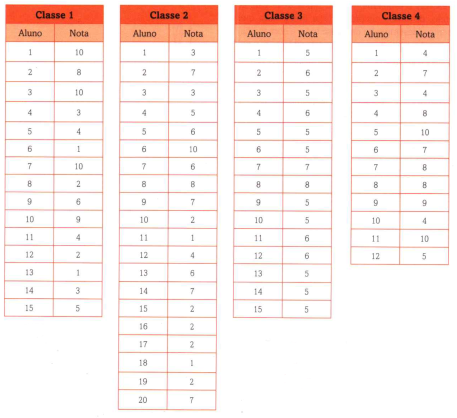
\includegraphics[width=1\linewidth]{6FMA11_imagens/imagem1}
	O professor prometeu um prêmio para a sala de melhor desempenho na prova, mas após comparar os resultados, mais de uma sala se achou no direito de reivindicar o prêmio.
	\begin{itemize}
		\item A classe 1 argumentava que seu desempenho era melhor, pois teve a maior quantidade de notas 10.
		\item A classe 2 achava justo o prêmio ser dela, pois ao somar todas as notas era dela a maior soma.
		\item A classe 3 tinha certeza de que o prêmio era dela, pois nenhum de seus alunos teve nota inferior a 5.
	\end{itemize}
	\noindent\textsubscript{-----------------------------------------------------------------------------------------------------------------------------------------------------------}
	\begin{multicols}{2}
		\begin{enumerate} 
			\item Na sua opinião, qual classe deve receber o prêmio e por quê? \\\\\\\\\\\\\\
			Observando com mais atenção, podemos chegar à conclusão de que os argumentos de todas as classes são falhos. \\
			O argumento da classe 1 leva em conta apenas o desempenho de alguns alunos e não da classe toda. \\
			O argumento da classe 2 também está errado, pois se uma sala tivesse mil alunos e todos tivessem tirado nota 1, a soma seria mais alta, apesar do péssimo desempenho da classe. \\
			E, finalmente, o argumento da classe 3 também pode ser questionado. Uma classe com a mesma quantidade de alunos que a classe 3 e que tenha apenas uma nota inferior a 5 pode ter um desempenho geral melhor que o da classe 3 (imagine que todas as outras notas da classe fossem 10). \\
			Para resolver o problema de qual classe deve ganhar o prêmio, devemos encontrar uma única nota que represente o desempenho da classe toda: a nota média. \\
			A soma das notas dos 15 alunos da classe 1 é 78. Dividindo a soma das notas pelo total de alunos obtemos $\frac{78}{15}$ = 5,2, que é a nota média da classe 1. \\
			Em Matemática, a operação que acabamos de fazer é chamada de \textbf{média aritmética}. \\
			A \textbf{média aritmética} de um conjunto com $n$ informações numéricas é obtida pela razão entre a soma dos valores numéricos dos elementos do conjunto e a quantidade $n$ de informações.
			\item Calcule a média aritmética das notas das classes 2, 3 e 4, e decida qual deve ganhar o prêmio. \\\\\\\\\\\\\\\\\\\\\\\\\\
			%40 a 43
			\item Calcule a média aritmética dos números: 
			\begin{enumerate}[a)]
				\item 4 e 16. \\\\\\\\\\
				\item 140 e 160. \\\\\\\\\\
				\item 21, 18 e 24. \\\\\\\\\\
				\item 3, 4 e 5. \\\\\\\\\\
				\item 10, 20, 30 e 40. \\\\\\\\\\
			\end{enumerate}
			\item Calcule a média aritmética dos números:
			\begin{enumerate}[a)]
				\item 1, 2 e 3. \\\\\\\\\\
				\item 3, 4 e 5. \\\\\\\\\\
				\item 5, 6 e 7. \\\\\\\\\\
				\item 7, 8 e 9. \\\\\\\\\\
			\end{enumerate}
			A qual conclusão se pode chegar sobre a média aritmética de três números naturais consecutivos? \newpage
			\item Na cidade de Curitiba foram registradas em uma determinada semana do último inverno as seguintes temperaturas médias diárias: \\
			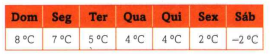
\includegraphics[width=1\linewidth]{6FMA11_imagens/imagem2} \\
			Qual foi a temperatura média naquela semana? \\\\\\\\\\
			\item Calcule a média aritmética dos números:
			\begin{enumerate}[a)]
				\item 1 e 3. \\\\\\\\\\
				\item 4 e 6. \\\\\\\\\\
				\item 5 e 7. \\\\\\\\\\
				\item 8 e 10. \\\\\\\\\\
				\item 11 e 13. \\\\\\\\\\
			\end{enumerate}
			Você chegou a alguma conclusão? Qual?
		\end{enumerate}
		$~$ \\ $~$ \\ $~$ \\ $~$ \\ $~$ \\ $~$ \\ $~$ \\ $~$ \\ $~$ \\ $~$ \\ $~$ \\ $~$ \\ $~$ \\ $~$ \\ $~$ \\ $~$ \\ $~$ \\ $~$ \\ $~$ \\ $~$ \\ $~$ \\ $~$ \\ $~$ \\ $~$ \\ $~$ \\ $~$ \\ $~$ \\ $~$ \\ $~$ \\ 
	\end{multicols}
\end{document}